\begin{center}
\Huge
Vækst af eksponentialfunktioner
\end{center}
\section*{Vækst af lineære funktioner}
\stepcounter{section}

Da vi arbejdede med lineær vækst så vi, at den øgedes ved at lægge hældningen $a$ til funktionsværdien hver gang vi øgede $x$-værdien med 1. 
\begin{exa}
	En container fyldes med sand. Containeren vejer 700kg og den fyldes med 1000kg sand i 
	timen. Denne situation kan beskrives ved den lineære funktion $f$ givet ved
	\begin{align*}
		f(x) = 1000x + 700,
	\end{align*}	 
	hvor $x$ betegner antal forløbne timer og $f$ er totalvægten af containeren. 
	Tegner vi denne model får vi
	\begin{figure}[H]
		\centering
		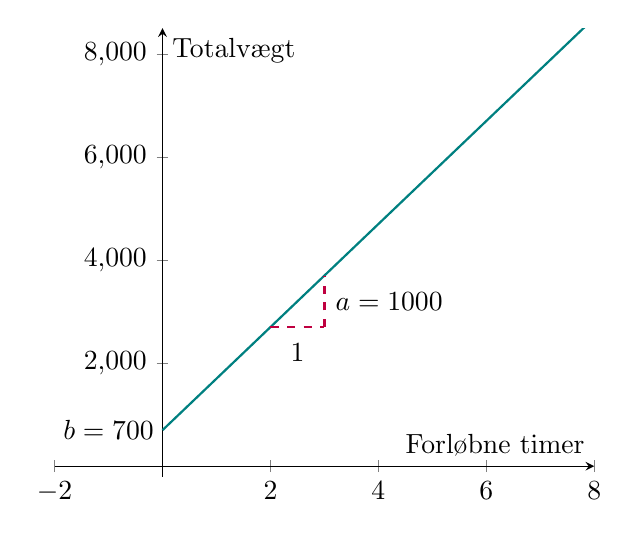
\begin{tikzpicture}
			\begin{axis}[
			axis lines = middle,
			 xmin = -2, xmax = 8, ymin = -200, ymax = 8500,
			 xlabel = {Forløbne timer}, ylabel = {Totalvægt}
			]
				\addplot[domain = 0:8, color = teal, thick] {1000*x + 700};
				\draw[dashed, color = purple, thick] (axis cs: 2,2700) -- (axis cs: 3,2700);
				\draw[dashed, color = purple, thick] (axis cs: 3,2700) -- (axis cs: 3,3700);						\node at (axis cs: 4.2, 3200) {$a = 1000$};
				\node at (axis cs: -1, 700) {$b = 700$};
				\node at (axis cs: 2.5,2200) {$1$};
			\end{axis}
		\end{tikzpicture}
		\caption{Totalvægt af container}
	\end{figure}
	Vi kan også beskrive dette ved en tabel. Tabel \ref{tab:sildebenlin} beskriver funktionen 
	$f$.
	\begin{figure}[H]
		\center
		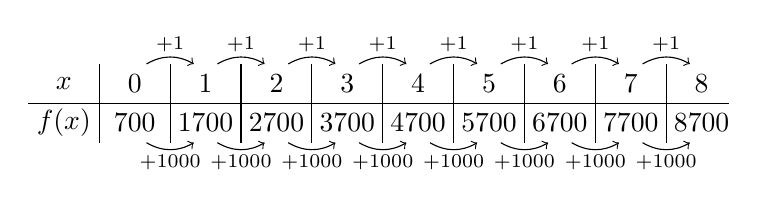
\begin{tikzpicture}
			\foreach \i in {0,...,8}{
			\draw (\i*0.9,0) -- (\i*0.9,1);
			}
			\draw (-0.9,0.5) -- (8,0.5);
			\foreach \i in {0,...,8}{
			\node at (\i*0.9+ 0.45,0.75) {$\i$};
			\node at (\i*0.9+0.45,0.25) {$\fpeval{1000*\i + 700}$};
			}
			\node at (-0.45,0.75) {$x$};
			\node at (-0.45,0.25) {$f(x)$};
			\foreach \i in {0,...,7}{
			\draw [->] (\i*0.9+0.6,1) to [out=30,in=150] (\i*0.9+1.2,1);
			\node at (\i*0.9+0.9,1.25) {$\scriptstyle+1$};
			\draw [->] (\i*0.9+0.6,-0) to [out=-30,in=-150] (\i*0.9+1.2,-0);
			\node at (\i*0.9+0.9,-0.25) {$\scriptstyle + 1000$};
			}
		\end{tikzpicture}
		\caption{Totalvægt af container}
		\label{tab:sildebenlin}
	\end{figure}
\end{exa}

\section*{Procentvis vækst}

Vi så sidst, at vi for at øge en størrelse $S$ med en fast procent $p$ skulle multiplicere 
$S$ med $(1 + \frac{p}{100})$. Skal vi eksempelvis øge 120 med 10 procent bestemmer vi
\begin{align*}
	120 \cdot 1.10 = 132.
\end{align*}

Ønsker vi at øge 120 med 10 procent to gange, så øger vi blot 132 med 10 procent igen. Så får vi
\begin{align*}
	132 \cdot 1.10 = 145.2.
\end{align*}

\begin{exa}
	En bestemt plantes vægt vokser med 10 $\%$ om ugen. Vi ønsker at opstille en lignende tabel
	 som Tabel \ref{tab:sildebenlin}, men med plantens vægt. Vi skal nu være opmærksomme på, at  
	 vi nu skal gange med $1.10$ hver gang der går en uge. Lad os sige, at planten vejer 200g i 
	 begyndelsen. Resultatet kan ses af Tabel \ref{tab:sildebenplante}.
	 \begin{figure}[H]
		\center
		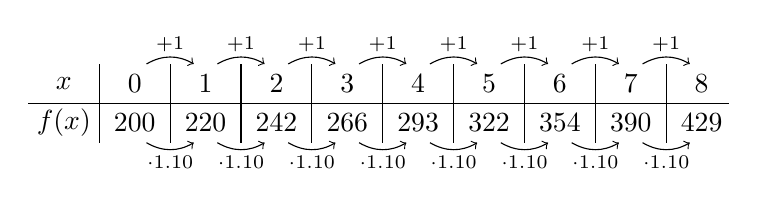
\begin{tikzpicture}
			\foreach \i in {0,...,8}{
			\draw (\i*0.9,0) -- (\i*0.9,1);
			}
			\draw (-0.9,0.5) -- (8,0.5);
			\foreach \i in {0,...,8}{
			\node at (\i*0.9+ 0.45,0.75) {$\i$};
			\node at (\i*0.9+0.45,0.25) {$\fpeval{round(200*(1.10)^\i,0)}$};
			}
			\node at (-0.45,0.75) {$x$};
			\node at (-0.45,0.25) {$f(x)$};
			\foreach \i in {0,...,7}{
			\draw [->] (\i*0.9+0.6,1) to [out=30,in=150] (\i*0.9+1.2,1);
			\node at (\i*0.9+0.9,1.25) {$\scriptstyle+1$};
			\draw [->] (\i*0.9+0.6,-0) to [out=-30,in=-150] (\i*0.9+1.2,-0);
			\node at (\i*0.9+0.9,-0.25) {$\scriptstyle \cdot 1.10$};
			}
		\end{tikzpicture}
		\caption{Vægt af plante}
		\label{tab:sildebenplante}
	\end{figure}
\end{exa}

Ud fra dette eksempel vil vi definere begrebet eksponentialfunktion.
\begin{defn}[Eksponentialfunktion]
	Lad $a,b>0$. Så definerer vi en funktion $f$ på formen 
	\begin{align*}
		f(x) = b\cdot a^x
	\end{align*}
	til at være en \textit{eksponentialfunktion} med \textit{begyndelsesværdi} $b$ og 
	textit{fremskrivningsfaktor} $a$. 
\end{defn}

Det er ikke svært at se, hvorfor $b$ kaldes for begyndelsesværdien thi
\begin{align*}
	f(0) = b\cdot a^0 = b\cdot 1 = b.
\end{align*}

\begin{exa}\label{exa:exa1}
Lad os betragte delingen af en bakterie. Vi starter med 1 bakterie, der efter én time er 2 bakterier, efter 2 timer er 4 bakterier, efter 3 timer er 8 bakterier osv. Denne situation kan beskrives ved eksponentialfunktionen $f(x)$ givet ved
\begin{align*}
f(x) = 2^x.
\end{align*}
De første 10 funktionsværdier kan ses af Fig. \ref{fig:sildebenfold}
\begin{figure}[H]
\center
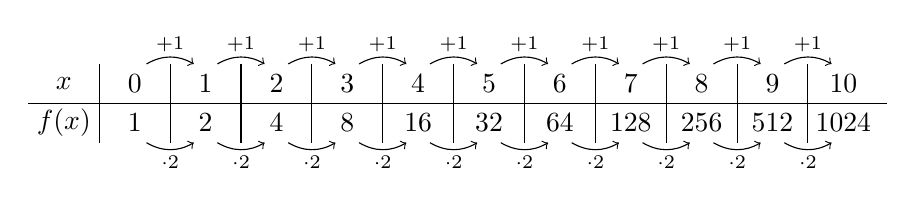
\begin{tikzpicture}
\foreach \i in {0,...,10}{
\draw (\i*0.9,0) -- (\i*0.9,1);
}
\draw (-0.9,0.5) -- (10,0.5);
\foreach \i in {0,...,10}{
\node at (\i*0.9+ 0.45,0.75) {$\i$};
\node at (\i*0.9+0.45,0.25) {$\fpeval{2^{\i}}$};
}
\node at (-0.45,0.75) {$x$};
\node at (-0.45,0.25) {$f(x)$};
\foreach \i in {0,...,9}{
\draw [->] (\i*0.9+0.6,1) to [out=30,in=150] (\i*0.9+1.2,1);
\node at (\i*0.9+0.9,1.25) {$\scriptstyle+1$};
\draw [->] (\i*0.9+0.6,-0) to [out=-30,in=-150] (\i*0.9+1.2,-0);
\node at (\i*0.9+0.9,-0.25) {$\scriptstyle\cdot 2$};
}
\end{tikzpicture}
\caption{De første ti funktionsværdier af $f$, der beskriver antallet af bakterier. }
\label{fig:sildebenfold}
\end{figure}
På Fig \ref{fig:flagxfold} kan grafen for $f$ ses. 
\begin{figure}[H]
\center
\begin{tikzpicture}
	\begin{axis}[axis lines=left,
		xlabel = {$x$ (Timer)},
		ylabel = {$y$ (Bakterier)}]
		\addplot[color=blue!40,thick, domain=0:10,samples=1000]{2^x};
	\end{axis}
\end{tikzpicture}
\caption{Antal bakterier som funktion af tiden}
\label{fig:flagxfold}
\end{figure}
\end{exa}
Inspriret af Eksempel \ref{exa:exa1} vil vi se på, hvordan eksponentiel vækst udvikler sig. Vi husker på, at en eksponentialfunktion $f$ kan skrives på formen
\begin{align*}
f(x) = b\cdot a^x.
\end{align*}
Ser vi på Fig. \ref{fig:sildebenfold}, så kan vi se, at vi i det tilfælde øger $f(x)$ med en faktor $2$, når vi øger $x$ med 1. Tilsvarende vil vi øge generel eksponentiel vækst med en faktor $a$, når vi øger $x$ med 1. Faktoren $a$ kaldes for fremskrivningsfaktoren. Vi kan se dette fænomen af Fig. \ref{fig:sildegen}
\begin{figure}[H]
\center
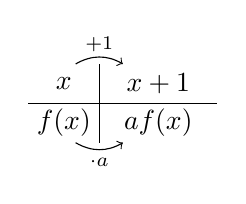
\begin{tikzpicture}
\foreach \i in {0}{
\draw (\i*0.9,0) -- (\i*0.9,1);
}
\draw (-0.9,0.5) -- (1.5,0.5);
\foreach \i in {0}{
\node at (\i*0.9+ 0.75,0.75) {$x+1$};
\node at (\i*0.9+0.75,0.25) {$af(x)$};
}
\node at (-0.45,0.75) {$x$};
\node at (-0.45,0.25) {$f(x)$};
\foreach \i in {0}{
\draw [->] (\i*0.9-0.3,1) to [out=30,in=150] (\i*0.9+0.3,1);
\node at (\i*0.9,1.25) {$\scriptstyle+1$};
\draw [->] (\i*0.9-0.3,-0) to [out=-30,in=-150] (\i*0.9+0.3,-0);
\node at (\i*0.9,-0.25) {$\scriptstyle\cdot a$};
}
\end{tikzpicture}
\caption{Udvikling af eksponentiel vækst.}
\label{fig:sildegen}
\end{figure}
Det er ikke svært at vise, at dette rent faktisk er sandt. Betragter vi
\begin{align*}
f(x+1) = ba^{x+1} = ba^xa = af(x),
\end{align*}
så ses det, at eksponentialfunktioner har en sådan udvikling. 
\begin{defn}[Vækstrate og fremskrivningsfaktor]
	For en eksponentialfunktion $f$ givet ved
	\begin{align*}
		f(x) = b\cdot a^x
	\end{align*}
	kaldes $a$ for \textit{fremskrivningsfaktoren.}
	Vi definerer desuden \textit{vækstraten} $r$ som
	\begin{align*}
		r = a -1.
	\end{align*}
\end{defn}

\subsection*{Opgave 1}

En person får en timeløn på $130$ kr. Han får hvert år en lønstigning på $20$kr i timen. Udfyld følgende tabel, der beskriver vedkommenes timeløn efter $x$ år
\begin{center}
	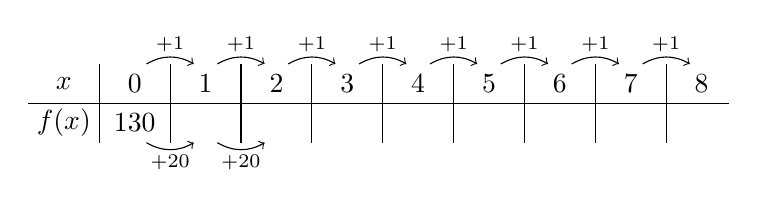
\begin{tikzpicture}
			\foreach \i in {0,...,8}{
			\draw (\i*0.9,0) -- (\i*0.9,1);
			}
			\draw (-0.9,0.5) -- (8,0.5);
			\foreach \i in {0,...,8}{
			\node at (\i*0.9+ 0.45,0.75) {$\i$};
			}
			\foreach \i in {0}{
			\node at (\i*0.9+0.45,0.25) {$\fpeval{20*\i + 130}$};
			}
			\node at (-0.45,0.75) {$x$};
			\node at (-0.45,0.25) {$f(x)$};
			\foreach \i in {0,...,7}{
			\draw [->] (\i*0.9+0.6,1) to [out=30,in=150] (\i*0.9+1.2,1);
			\node at (\i*0.9+0.9,1.25) {$\scriptstyle+1$};
			}
			\foreach \i in {0,...,1}{
			\draw [->] (\i*0.9+0.6,-0) to [out=-30,in=-150] (\i*0.9+1.2,-0);
			\node at (\i*0.9+0.9,-0.25) {$\scriptstyle + 20$};
			}
	\end{tikzpicture}
\end{center}

\begin{enumerate}[label=\roman*)]
	\item Brug tabellen til at bestemme personens timeløn efter 6 år
	\item Bestem en funktionsforskrift for $f$ der beskriver personens løn efter $x$ år.
\end{enumerate}

\subsection*{Opgave 2}

En person får om måneden 30000 i løn. Vedkommende får årligt en lønstigning på $4\%$. Udfyld følgende tabel, der beskriver vedkommenes månedsløn efter $x$ år

\begin{center}
	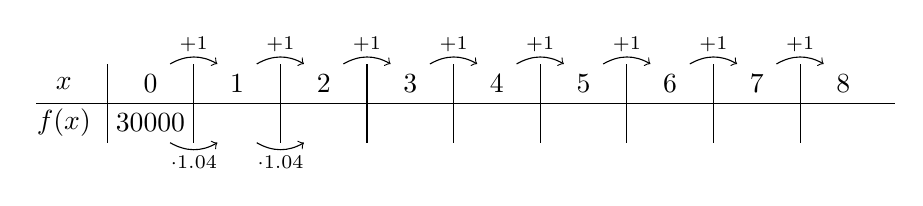
\begin{tikzpicture}
			\foreach \i in {0,...,8}{
			\draw (\i*1.1,0) -- (\i*1.1,1);
			}
			\draw (-0.9,0.5) -- (10,0.5);
			\foreach \i in {0,...,8}{
			\node at (\i*1.1+ 0.55,0.75) {$\i$};
			}
			\foreach \i in {0}{
			\node at (\i*1.1+0.55,0.25) {$\fpeval{round(30000*(1.04)^\i,0)}$};
			}
			\node at (-0.55,0.75) {$x$};
			\node at (-0.55,0.25) {$f(x)$};
			\foreach \i in {0,...,7}{
			\draw [->] (\i*1.1+0.8,1) to [out=30,in=150] (\i*1.1+1.4,1);
			\node at (\i*1.1+1.1,1.25) {$\scriptstyle+1$};
			}
			\foreach \i in {0,...,1}{
			\draw [->] (\i*1.1+0.8,-0) to [out=-30,in=-150] (\i*1.1+1.4,-0);
			\node at (\i*1.1+1.1,-0.25) {$\scriptstyle  \cdot 1.04$};
			}
	\end{tikzpicture}
\end{center}

\begin{enumerate}[label = \roman*)]
	\item Hvad er personens månedsløn efter 7 år?
	\item Hvordan noterer vi, at vi har ganget med det samme tal flere gange? Hvad skal vil 
	gange $30000$ med, hvis vi gerne vil bestemme personens månedsløn efter 10 år?
	\item Har du en idé til, hvordan forskriften for funktionen, der beskriver
	personens løn efter $x$ år kunne se ud? Hvis ikke, så går du bare videre. 
	\item Tallet $1.04$ kaldes for \textit{fremskrivningsfaktoren}. Hvad ville fremskrivnings-
	faktoren være, hvis personens løn skulle stige med 2$\%$ om året?
	\item Hvad ville fremskrivningsfaktoren være, hvis personens løn skulle falde med $2\%$ om 
	året?
	\item Kan du gennemskue, hvad der skal gælde om fremskrivningsfaktoren, hvis personens løn 
	skal vokse? 
	\item Kan du gennemskue, hvad der skal gælde om fremskrivningsfaktoren, hvis personens løn 
	skal aftage?
\end{enumerate}

\subsection*{Opgave 3}

I en opløsning findes en bakteriekoloni, der hvert døgn tredobles i antal. Der er i starten af kolonien 200 bakterier.

\begin{enumerate}[label=\roman*)]
	\item Hvad skal antallet af bakterier ganges med hver gang der er gået ét døgn?
	\item Udfyld en tabel med antallet af bakterier efter de første 6 døgn.
	\item Udregn hvor mange procent antallet af bakterier stiger fra dag 2 til dag 3 samt fra 
	dag 3 til dag 4? Giver det mening?
\end{enumerate} 




\subsection*{Opgave 4}



\begin{enumerate}[label=\roman*)]
	\item En eksponentialfunktion $f$ er givet ved
	\begin{align*}
		f(x) = 1.3\cdot 0.97^x.
	\end{align*}
	Bestem fremskrivningsfaktoren og vækstraten for $f$. Afgør desuden hvor mange procent $f$ stiger/falder med, hvis $x$ øges med 1.
	\item En eksponentialfunktion $f$ er givet ved
	\begin{align*}
		f(x) = 1\cdot 2^x.
	\end{align*}
	Bestem fremskrivningsfaktoren og vækstraten for $f$. Afgør desuden hvor mange procent $f$ stiger/falder med, hvis $x$ øges med 1.
	\item En eksponentialfunktion $f$ er givet ved
	\begin{align*}
		f(x) = 9\cdot 1.34^x.
	\end{align*}
	Bestem fremskrivningsfaktoren og vækstraten for $f$. Afgør desuden hvor mange procent $f$ stiger/falder med, hvis $x$ øges med 1.
	\item En eksponentialfunktion $f$ er givet ved
	\begin{align*}
		f(x) = \sqrt{2}\cdot 5^x.
	\end{align*}
	Bestem fremskrivningsfaktoren og vækstraten for $f$. Afgør desuden hvor mange procent $f$ stiger/falder med, hvis $x$ øges med 1.
\end{enumerate}

\subsection*{Opgave 5}
a) En eksponentialfunktion $f$ er givet ved
\begin{align*}
	f(x) = 6.7\cdot 1.3^x.
\end{align*}
\begin{enumerate}[label=\roman*)]
	\item Bestem $f(4)$.
	\item Bestem $f(-3)$.
\end{enumerate}

b) En eksponentialfunktion $g$ har begyndelsesværdi $7$ og fremskrivningsfaktor $0.7$.
\begin{enumerate}[label=\roman*)]
	\item Opskriv forskriften for $g$. 
	\item Bestem $g(7)$. 
\end{enumerate}

\subsection*{Opgave 6}
\begin{enumerate}[label=\roman*)]
	\item Udfyld følgende tabel og opskriv derefter forskriften for eksponentialfunktionen $f$.
	\item Undersøg, om du har udfyldt tabellen korrekt ved at bestemme $f(10)$. 
\end{enumerate}

\begin{center}
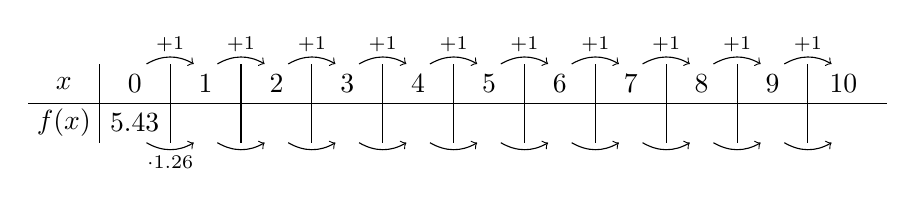
\begin{tikzpicture}
\foreach \i in {0,...,10}{
\draw (\i*0.9,0) -- (\i*0.9,1);
}
\draw (-0.9,0.5) -- (10,0.5);
\foreach \i in {0,...,10}{
\node at (\i*0.9+ 0.45,0.75) {$\i$};
}
\node at (0.45,0.25) {$5.43$};
\node at (-0.45,0.75) {$x$};
\node at (-0.45,0.25) {$f(x)$};
\foreach \i in {0,...,9}{
\draw [->] (\i*0.9+0.6,1) to [out=30,in=150] (\i*0.9+1.2,1);
\node at (\i*0.9+0.9,1.25) {$\scriptstyle+1$};
\draw [->] (\i*0.9+0.6,-0) to [out=-30,in=-150] (\i*0.9+1.2,-0);
}
\node at (0.9,-0.25) {$\scriptstyle\cdot 1.26$};
\end{tikzpicture}
\end{center}

\subsection*{Opgave 7}

\begin{enumerate}[label=\roman*)]
	\item Lad $f$ være givet ved
	\begin{align*}
		f(x) = 5\cdot 1.7^x.
	\end{align*}
	Hvor mange procent øges $f$ med, hvis $x$ øges med 2?
	\item Lad $f$ være givet ved
	\begin{align*}
		f(x) = b\cdot 0.77^x.
	\end{align*}
	Det oplyses, at $f(4) = 6.01$. Bestem $f(8)$. 
	\item Lad $f$ være givet ved
	\begin{align*}
		f(x) = 9.99 \cdot 1.05^x.
	\end{align*}
	Hvor meget skal $x$ øges med før $f$ fordobles?
\end{enumerate}


\subsection*{Opgave 8}
Hver gang vi folder et stykke papir, så vil antallet af papirlag fordobles. Antallet af lag kan beskrives af en eksponentialfunktion 
\begin{align*}
	f(x) = b\cdot a^x.
\end{align*}
\begin{enumerate}[label=\roman*)]
	\item Hvad er begyndelsesværdien og fremskrivningsfaktoren for $f$?
	\item Hvor mange lag har et stykke papir, hvis det er foldet 7 gange?
	\item Forestil dig, at du kan folde papiret lige så mange gange du har lyst. Hvor tykt er
	papiret, hvis du har foldet det 25 gange?
 	\item Hvis ét lag papir er 0.1mm tykt, hvor tykt er dette stykke foldede papir?
	\item Hvor mange gange skal vi folde papiret, for at det bliver 1km tykt?
\end{enumerate}
\subsection*{Opgave 9}
\begin{enumerate}[label=\roman*)]
\item En bakteriekoloni indeholder til tid $t=0$ $B_0 = 100.000$ bakterier. En bakterie deler sig i gennemsnit 1 gang per 4. time, og bakteriekolonien har ubegrænset plads. Beskriv antallet af bakterier som funktion af tiden i timer. Hvor mange bakterier er der i kolonien efter et døgn? Hvornår er der 1 mia. $(10^9)$ bakterier i kolonien?
\item Et glas vand stilles i et rum, og temperaturen i vandet antages at kunne beskrives ved
\begin{align*}
H(t) = 70\cdot(0.97)^t,
\end{align*}
hvor $H(t)$ beskriver temperaturen i grader celcius og $t$ betegner tiden i minutter. Hvor varmt er vandet, når det stilles ind i rummet? Hvor varmt er det efter 5 minutter? Hvor varmt er der i rummet i følge modellen. 
\end{enumerate}

\subsection*{Opgave 10}
\begin{enumerate}[label=\roman*)]
\item Bevis, at hvis vi øger $x$ med 2 i en eksponentialfunktion $f(x)$, så tilsvarer dette at øge $f(x)$ med en faktor $a^2$. Hvad hvis vi øger $x$ med $3$?
\item Bevis, at hvis vi øger $x$ med $n$ i en eksponentialfunktion $f(x)$, så tilsvarer dette at øge $f(x)$ med en faktor $a^n$.
\end{enumerate}